\chapter{\textcolor{red}{Az alkalmazás működése}}
\label{ch:mukodes}
Ebben a fejezetben bemutatásra kerül az alkalmazás működése felhasználói szempontból, bővebben kifejtve \aref{sec:projektrol:funkcionalitasok}. fejezetben említett funkcionalitásokat, a szerző által implementáltakra fókuszálva. 
\begin{figure}
  \centering
  \pgfimage[width=0.9\linewidth]{images/emigrated_terkep}
  \caption{Az E-migrated főoldalán bejelentkezett felhasználók számára láthatóak a felhasználói információk.}
  \label{fig:emigrated_terkep}
\end{figure}


A webes felület főoldalán látható egy Google Maps térkép, amelyen gyűjtőpontok jelzik, hogy mely régióból hány regisztrált felhasználója van az alkalmazásnak.

Közelítve a térképet, ezek a gyűjtőpontok felbomlanak további térképjelzőkre, részletesebben mutatva a régiókat. Egy nem bejelentkezett felhasználó nem lát információt a regisztrált tagokról, csupán annyit, hogy mely zónából hányan vannak csatlakozva a rendszerhez. 


Ahogyan a \ref{fig:emigrated_terkep}. ábrán is látható, egy bejelentekezett felhasználó viszont már megjelenítheti az adott gyűjtőpont alatt lakó személyek adatait: nevüket, e-mail címüket, profilképüket, illetve nevükre kattintva át is navigálhat az adott felhasználó publikus profiljára. Ha egy gyűjtőpont alatt többen laknak mint három, akkor a gyűjtőpontra kattintva az ablak jobb oldalán megjelenik egy keskeny sáv a felhasználók adataival, ha hárman vagy annál kevesebben vannak, akkor a térképen jelenik meg, egy felügró ablak, mutatva az információkat. 


Az E-migrated alkalmazás fő menüje az ablak felső részén kapott helyet. Itt tudják a felhasználók kiválasztani a kívánt nyelvet, illetve itt tudnak bejelentkezni. A \textit{Bejelentkezés} menüpont alatt választhatnak a hagyományos bejelentkezés vagy a Facebook-kal való bejelentkezés között, illetve kérhetnek meghívót, amennyiben még nem regisztráltak. \textit{Bejelentkezés Facebook-kal} gombra kattintva csak akkor tudnak bejelentkezni, ha ezen a szociális hálón keresztül regisztráltak a rendszerbe, vagy a későbbiekben hozzákapcsolták a fiókjukat az E-migrated profiljukhoz, különben hibaüzenetet kapnak. 
\begin{figure}
  \centering
  \pgfimage[width=0.5\linewidth]{images/emigrated_meghivo_igenyles}
  \caption{Meghívó igénylése}
  \label{fig:emigrated_meghivo_igenyles}
\end{figure}

Meghívót, ahogyan a \ref{fig:emigrated_meghivo_igenyles}. ábra is mutatja, egy e-mail cím és egy rövid motivációs levél megadásával, illetve egy önéletrajz feltöltésével igényelhetnek a vendégek.
\begin{figure}[!b]
  \centering
  \pgfimage[width=0.8\linewidth]{images/osszes_bejegyzes}
  \caption{Bejegyzések böngészése.}
  \label{fig:osszes_bejegyzes}
\end{figure}



A bejelentkezett felhasználók számára a menü további menüpontokkal bővül. Megjelennek a \textit{Meghívó küldése}, illetve \textit{Bejegyzések} menüpontok, valamint a \textit{Bejelentkezés} menüpont helyett most a felhasználó neve lesz feltüntetve. 


A \textit{Bejegyzések} menüpont alatt a felhasználók böngészhetik a mások által közzétett bejegyzéseket, melyek egymás után, a görgetés során, folyamatosan töltődnek be (\ref{fig:osszes_bejegyzes}. ábra). Ha egy bejegyzés szövege hosszú, a bejegyzés nem jelenik meg egész terjedelmében, csupán egy része, a teljes bejegyzés a \textit{tovább} linkre kattintva  jeleníthető meg. A baloldali menüből kiválasztva a megfelelő menüpontot a felhasználók megtekinthetik a saját bejegyzéseiket, amelyeket akár  törölhetnek is, így azok többé nem lesznek láthatóak mások számára.


A \textit{Saját Profilom} menüpont alatt, melyet a saját nevükre kattintva jeleníthetnek meg \aref{fig:fiok_torlese}. képen látható nézet jelenik meg, baloldalon egy menüvel, melynek fejlécén a profilképük látható. Itt szerkezthetik a profiljuk különböző adatait, hozzárendelhetik az E-migrated fiókjukhoz a Facebook profiljukat, illetve törölhetik a fiókjukat. Ha valaki hozzárendelte a Facebook profilját az eredeti, E-migrated profiljához, attól a pillanattól kezdve bejelentkezhet Facebook segítségével is. A Facebook-kal regisztrált felhasználók itt állíthatnak be egy E-migrated account-ot, ha ezentúl szeretnék, hogy legyen a rendszerhez egy felhasználónevük és egy jelszavuk.

Profil törlése során a felhasználók két lehetőség közül választhatnak. Kérhetik, hogy fiókjuk törlése során törlődjön az összes általuk létrehozott bejegyzés is, vagy dönthetnek a bejegyzéseik megtartása mellett, hogy azok továbbra is elérhetőek legyenek a többi felhasználó számára. Ha a második lehetőséget választják az összes bejegyzésük hozzá lesz rendelve egy névtelen felhasználóhoz, így továbbra is böngészhető és visszakereshető marad a közösség többi tagja részére.
\begin{figure}
  \centering
  \pgfimage[width=0.8\linewidth]{images/fiok_torlese}
  \caption{Profil törlése során a felhasználók két lehetőség közül választhatnak, kérhetik, hogy fiókjuk törlése során törlődjön az összes általuk létrehozott bejegyzés is, vagy dönthetnek a bejegyzéseik megtartása mellett.}
  \label{fig:fiok_torlese}
\end{figure}

Az adminisztrátorok számára lehetőség nyílik váltani az általános menü és az adminisztrátor menü között. A számukra készített menü öt menüpontot tartalmaz: \textit{Szerkesztés, Felhasználók}, az adminisztrátor neve, \textit{Nyelv} és \textit{Váltás felhasználói módba}.

A \textit{Szerkesztés} menüpont alatt (\ref{fig:admin}. ábra) a bal oldali menüből kiválasztva a megfelelő menüpontot, megtekinthetik a beérkezett meghívó kéréseket, ezeket egy rövid üzenet kíséretében elfogadhatják, elutasíthatják vagy törölhetik. Ha pozitívan bírálnak el egy meghívó igénylést, a kérésben megadott e-mail címre, egy automatikusan renderelt üzenet küldődik, amelyhez az adminisztrátor személyes üzenetet is csatolhat, és ezt az e-mailt megnyitva az igénylő regisztrálhat a rendszerbe. Amennyiben elutasítanak egy kérést, szintén kap az igénylő egy üzenetet a megadott címre.

A \textit{Felhasználók} menüpont lehetőséget nyújt a felhasználók kilistázására (\ref{fig:admin}. ábra), megadva, hogy egy oldalon hány felhasználót szeretnének megjeleníteni, név szerinti keresésre, illetve itt tud az adminisztrátor felfüggeszteni vagy újra aktiválni egy felhasználói fiókot, megindokolva döntését. A felfüggesztett felhasználó e-mailben kap értesítést fiókja felfüggesztéséről és egészen addig, míg újra nem aktiválják a profilját nem tud bejelentkezni.


\begin{figure}[t]
    \centering
    \begin{minipage}{0.49\linewidth}
        \centering
        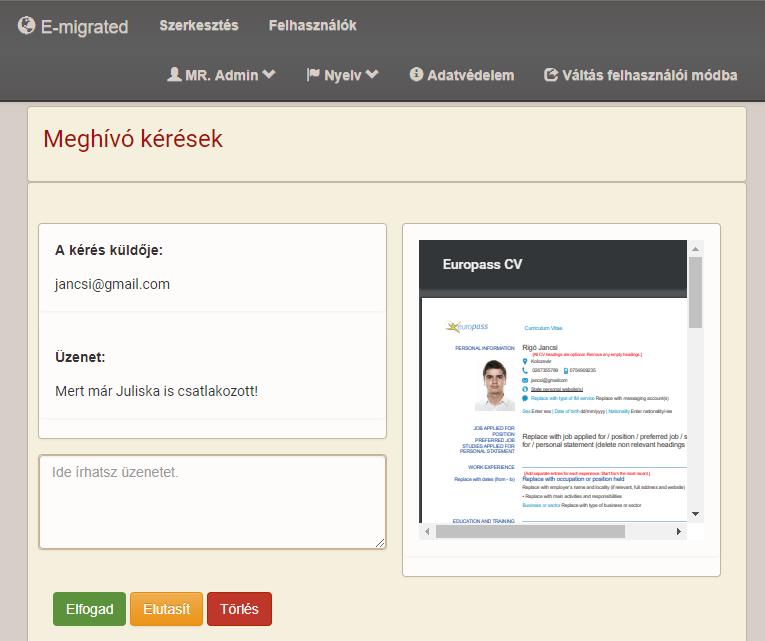
\includegraphics[height=0.83\linewidth]{images/meghivo_keres_admin}
    \end{minipage}
    \begin{minipage}{0.49\linewidth}
        \centering
        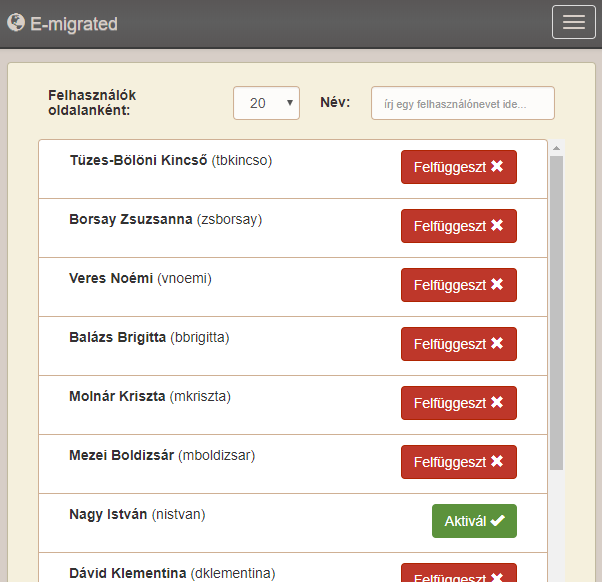
\includegraphics[height=0.83\linewidth]{images/admin_list_user}
    \end{minipage}
    \vspace*{3mm}
    \caption{A bal oldali képen láthatóak a beérkezett meghívó kérések, amelyeket az adminisztrátorok egy rövid üzenet kíséretében elfogadhatnak, elutasíthatnak vagy törölhetnek. A jobb oldali képen láthatóak az adminisztrátor által kilistázott felhasználók, itt függeszthetik fel a felhasználókat és kereshetnek közöttük név szerint. }
    \label{fig:admin}
\end{figure}











